\graphicspath{{figures/discussion}}
\section{Discussion}

%do the results we get for the two corner plots make sense knowing what we already know. Which grid is "better"?

%where are our degeneracies 

%does it agree with in general what an AGN is expected to look like (large wind etc) and then also does it look like how we expect NGC 3783 to look like.


% what are the things we need to do to the code to mkae it better.


% maybe make a table of "this study found this, then this study found this, and our study found this" in terms of parameters.

\label{sec:discussion}

\subsection{Comparison to Other Models of NGC 3783}

\begin{table*}
    \caption{Comparison of parameter estimates from different studies of NGC 3783. The first five columns show estimates from previous studies using different methods, while the last two columns show the estimates from this work using TORMAC with a torus only model and a torus plus polar bi-cone model.}
    \label{tab:param_comparison}
    \centering
    \begin{tabularx}{\textwidth}{l{c}*{6}{>{\centering\arraybackslash}X}}
    \hline
    & \cite{honig_dusty_2017} & \cite{gravity_collaboration_central_2021} & \cite{lyu_polar_2018} & \cite{bentz_detailed_2021} & \cite{fischer_determining_2013} & This Work (Torus Only) & This Work (Torus + Polar)\\
    \hline
    \Y & N/A & N/A & 500 & N/A& N/A & \\
    \hline
    \sig & <24\degree & 50-13 & N/A & 41-25 & N/A & \\
    \hline
    \p & -1 - 0 & incomparable & 0-1 & incomparable& N/A & \\
    \hline
    \vff & N/A & N/A & N/A & N/A & N/A & \\
    \hline
    \inc & 15-60\degree & 39-13\degree & 30-12\degree & 22-11\degree & 15\degree & \\
    \hline
    \Ypol & N/A & N/A & N/A & N/A & $\approx 2000$ & \\
    \hline
    \sigpol & N/A & N/A & N/A & N/A & 5\degree & \\
    \hline
    \ppol & >1 & N/A & N/A & N/A & N/A & \\
    \hline
    \vffpol & N/A & N/A & N/A & N/A & N/A & \\
    \hline
    \open & N/A & N/A & N/A & N/A & 50\degree & \\
    \hline
    \end{tabularx}
\end{table*}
% 
\par Our dust sublimation radius is 0.028pc \zach{also will need to explain why this is so small} which is based on a bolometric luminosity of $9.38\times10^{43}$ erg/s \zach{Need a citation for this!} and a dust sublimation temperature of 1500K.

\par \cite{hoenig_dust_2013} found that the mid-IR size of the wind is about 4.23 by 1.42 pc. This corresponds to a Y of .
\par \cite{gravity_collaboration_central_2021} found that the near-IR emission extends to a radius of \~0.07pc, and we compare this value with the RWD of our results.

\par Parameter estimates from this technique tend to correlate with predictions made by other methods. IR interferometric observations predict that the torus component of the dust has an inclination that is close to face-on to the observer (\inc $< 40\degree$) and a radial extent of \~0.07pc for the hot inner edge of the dust \citep{gravity_collaboration_central_2021}.  Kinematic simulations of NGC 3783 find a best fit to a polar bi-cone roughly perpendicular to the torus ($i_{\text{pol}} \approx 60$-$75\degree$ with $i_{\text{tor}} \approx 35$-$40\degree$, an offset of \~65-$85\degree$) with \sigpol $\approx 7$-$10\degree$, and a half opening angle of \~30-$50\degree$ \citep{fischer_determining_2013}\zach{; Müller-Sánchez et al. 2011}. Our models tend to suggest that higher inclination solutions may be allowable, but otherwise our findings are consistent with their results. Dust continuum SED models presented in Hönig and Kishimoto (2017) favor moderate inclinations between $15\degree$ and $60\degree$, \p values between –1 and 1, and \ppol $> 1$.


\par In the previous section, we examined the posterior distributions for the structure and geometry of a two component (torus and polar bi-cone) dust distribution model. We found that by increasing the complexity of the model grids used to perform the MCMC search, we were able to better model the IR response of NGC 3783. 
\par \cite{hoenig_dust_2013} found that the mid-IR size of the wind is about 4.23 by 1.42 pc.
\subsection{Parameter Estimation of NGC 3783}
\par We find that not all tested parameters have equal impact on the best fit IR response light curve, and are thus more difficult to constrain using this technique. Of the parameters that do most strongly impact the response light curve, we have yet to constrain only some. \zach{General statement not super useful here. This paragraph almost feels like it should be at the end of this subsection}
\par We consistently find the strongest constraints for \p (\~0) and \ppol (\~0), the radial cloud distribution power law indices. Lower \p values tend to result in light curves that respond on too short a time delay resulting in a light curve that is too “sharp”. This is likely due to most of the responding clouds being very close to the dust sublimation radius. Conversely, higher \p values tend to overly smooth the resulting light curve, with the same justification as for low \p values.  
\par The inclination (\inc) of the distribution is also generally well constrained to moderate inclinations ($30\degree$-$60\degree$), with the caveat that completely edge-on models (\inc $=90\degree$) were excluded as priors on the final set of models as they are generally unphysical to reverberation map. Performing reverberation mapping relies on the observer’s view of the central source being optically thin to the dust. In edge-on models, the central source would be completely obscured by the torus. These edge-on models, under certain conditions, resulted in degeneracies with models with other less extreme inclinations, motivating their exclusion. We find that inclination has more complex relationships with the other parameters, particularly the opening angle \open. This complexity can likely be attributed to discontinuities between optically thin and optically thick lines of sight to the inner regions of the dust, where the response is strongest.
\par We find that model grids tend to favor smaller \Y values. Hot dust at approximately 1000-2000K responds most strongly in the near-IR H and K bands. Only dust close to the dust sublimation radius ($\lesssim2R_d$) can reach these temperatures on their illuminated side, suggesting that the best fit \Y and \Ypol values we find may be more closely related to controlling the overall volume of the dust distribution and thus the cloud sizes. This also suggests that it may be possible to use this technique to further constrain the dust distribution at larger radii using light curves at longer wavelengths. 
We find that across model grids, \sig and \sigpol have a proportionally smaller impact on the response light curve and have not been constrained by our MCMC search. Comparing light curves where \sig and \sigpol are varied, the shorter timescale features tend to be muted as \sig and \sigpol increase. However, in further investigations, we would expect the angular width to also relate to the inclination in a similar way to \open. \zach{General ideas for this section: Could definitely figure out parameter importances!}

% \begin{figure}
%  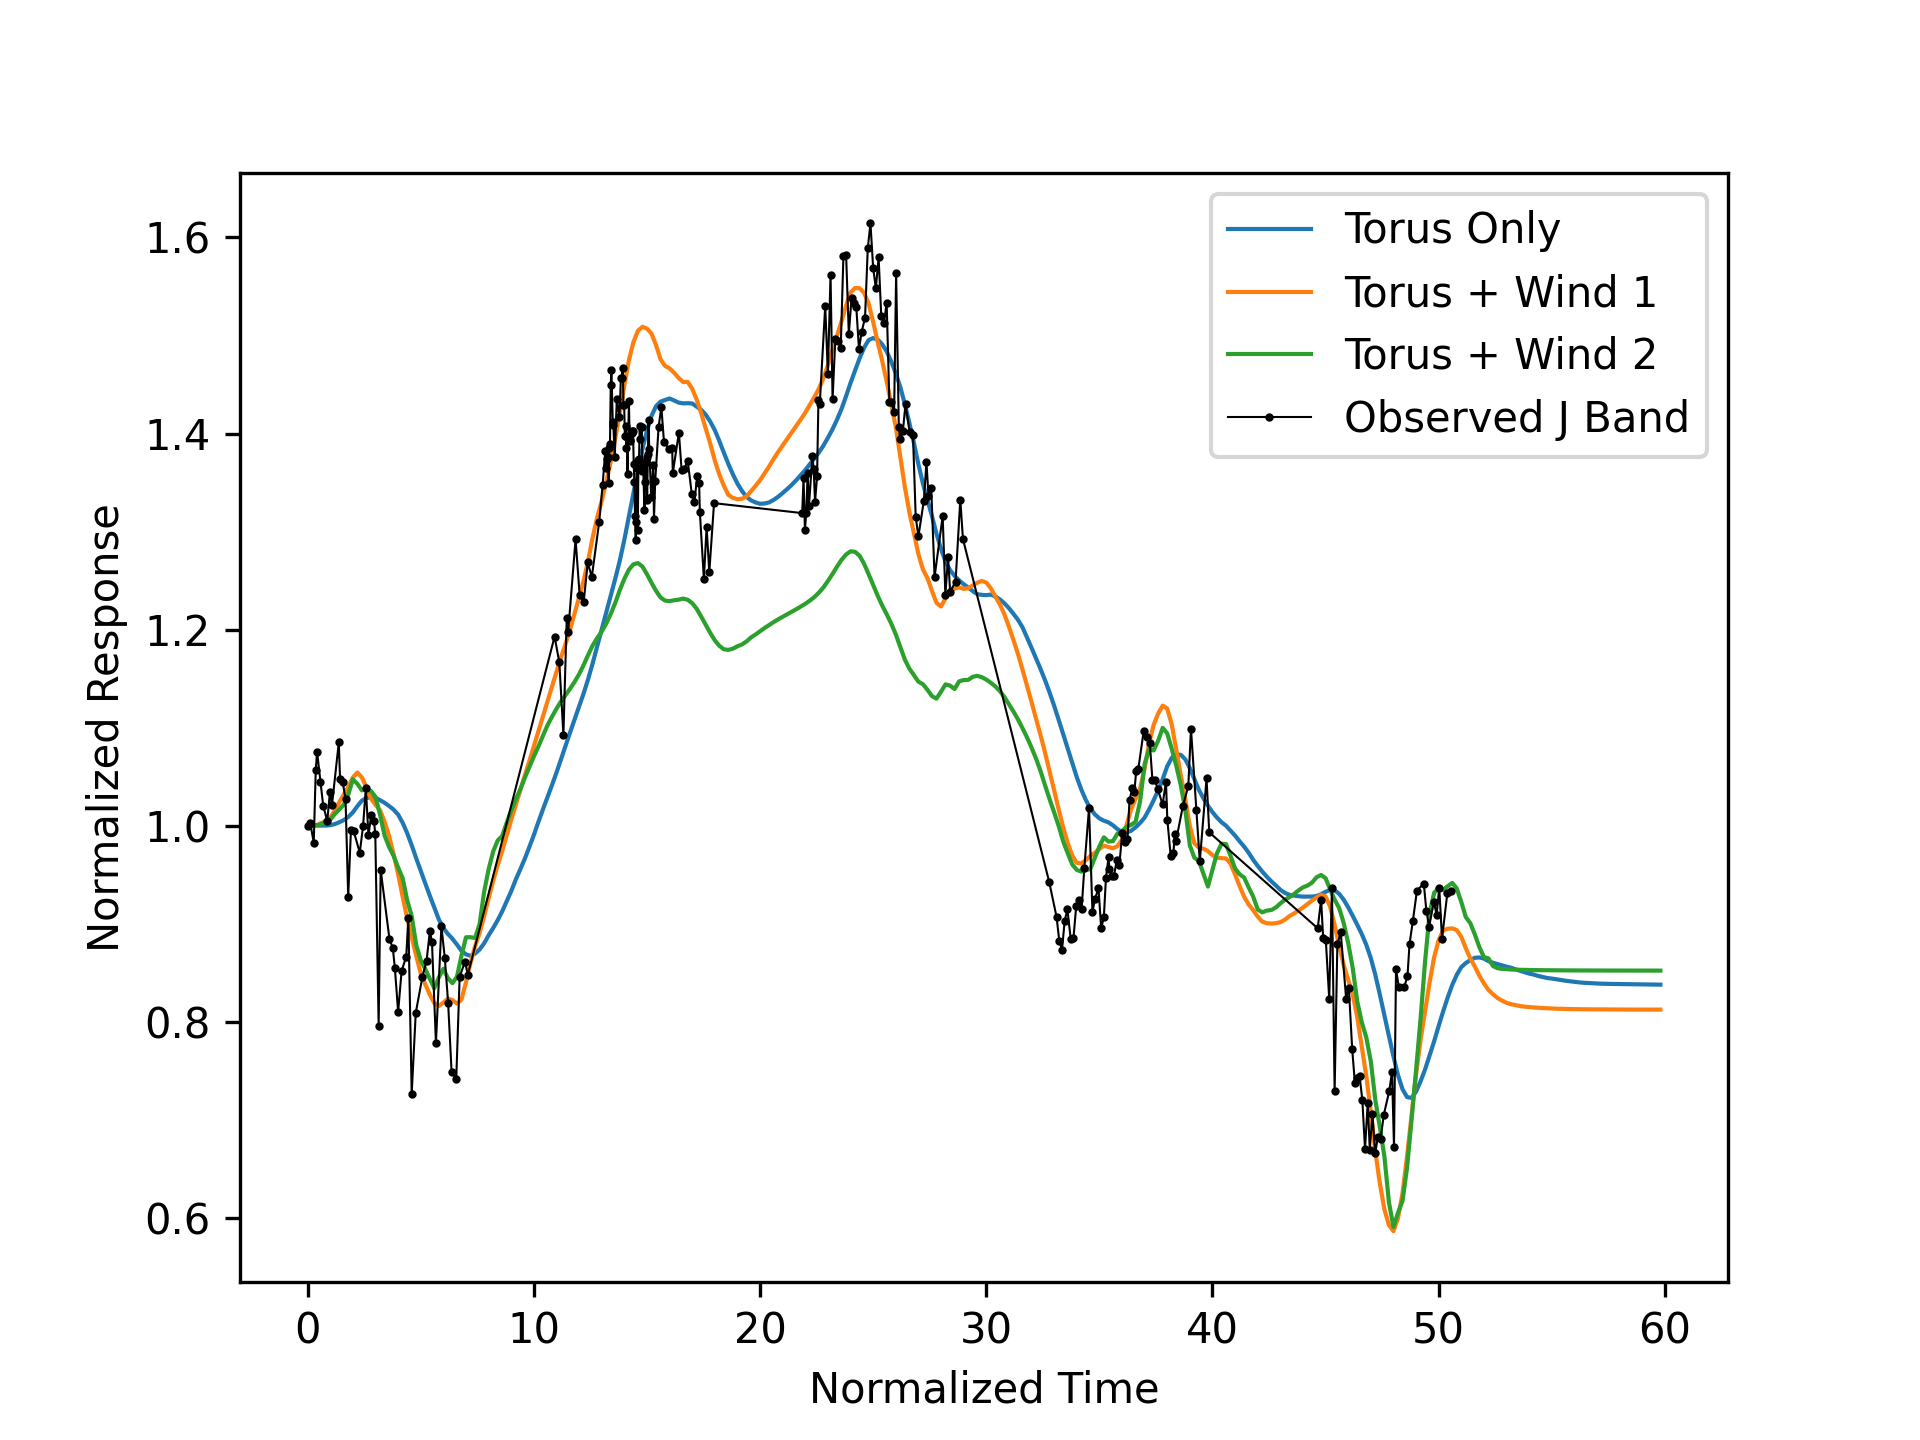
\includegraphics[width=\columnwidth]{modelcomparison.png}
%  \caption{Full TORMAC simulated responses for the best fit torus only model, the best fit torus and bi-cone model (Torus + Wind 1) and the same parameters but with the p parameter modified from 0 to -2 (Torus + Wind 2). Observed 1.25µm data from Lira et al. (2011) is also shown.}
%  \label{fig:modelcomparison}
% \end{figure}

\begin{itemize}
    \item Previous works generally support the conclusions drawn from "Torus 1" of the variable wind model set.
    \item It seems that grids must be relatively finely sampled for the influence from a non-delta transfer function to be determined.
    \item The parameter space should only contain feasible models, as non-physical / generally unsupported models can cause degeneracy with feasible models. 
    % Talk about previous methods used and how ours is unique
    %This section is definitely missing a lot of stuff
\end{itemize}

\subsection{Limitations \& Future Work}
\label{sec:limitations}
\subsubsection{Saturation Effects}
\par We now discuss multiple effects which we classify as "saturation effects" as they all have similar effect on the resulting simulated response, namely, at high relative luminosities they each result in a stunting of the response (saturation) which results in significant deviation from the observed data. 
\par One such effect which is well understood is when clouds become a sufficiently large such that only a small number of clouds ($\lesssim100$) are able to react directly. This is typically caused by large volume filling factors, large y values, and exacerbated by negative p values. These models are nonphysical due to the clouds' large size particularly at close to the inner edge, but the parameters used may not be nonphysical. This could be addressed by introducing a new parameter to describe the radial dependence of cloud volume, or by significantly increasing the number of clouds in the simulation.
\par {\bf DESCRIBE THE DEVIATION IN FIGURE 5} It is hypothesized that this deviation is caused by the fact that TORMAC currently simulates dust sublimation as a function of temperature only, when in reality it is also a time dependent process. In reality, as clouds at the inner edge of the dust distribution are pushed inside of the expanding dust sublimation radius, the inner edge of the clouds (which receive the majority of the heating from the central source) begin to sublimate away, while the interior of the cloud raises in temperature. Instead, since TORMAC simply caps the front edge of the cloud at the dust sublimation temperature, the interior of the cloud is capped at a lower temperature than would be expected, resulting in a saturation of the clouds during periods of high emission from the disk. 
%Mention J band problem?
%discuss the sublimation saturation problem
\begin{itemize}
    \item Produce more models with similar parameters to those explored in the third set of models, and iteratively refining the results by adding more in-between models.
    \item Model dust sublimation as a function of luminosity and time, may influence the response at high luminosities
    \item Model the polar bi-cone as parabolic and or hyperbolic
    \item Introduce variable cloud size as a function of radius
\end{itemize}